\documentclass{beamer}
\usepackage{listings}
\lstset{
%language=C,
frame=single, 
breaklines=true,
columns=fullflexible
}
\graphicspath{{./Figures/}}
\usepackage{gensymb}
\usepackage{subcaption}
\usepackage{url}
\usepackage{tikz}
\usepackage{tkz-euclide} % loads  TikZ and tkz-base
\usepackage{unicode-math}
%\usetkzobj{all}
\usetikzlibrary{calc,math}
\usepackage{float}
\usepackage{extarrows}
\newcommand\norm[1]{\left\lVert#1\right\rVert}
\providecommand{\pr}[1]{\ensuremath{\Pr\left(#1\right)}}
\newcommand{\myvec}[1]{\ensuremath{\begin{pmatrix}#1\end{pmatrix}}}
\renewcommand{\vec}[1]{\mathbf{#1}}
\usepackage[export]{adjustbox}
\usepackage[utf8]{inputenc}
\usepackage{amsmath}
\usetheme{Boadilla}

\title{Ramsey 4.2-Tangent and Normal-Q.21}
\author{Vaibhav Chhabra - AI20BTECH11022}

\begin{document}
\begin{frame}
\titlepage
\end{frame}
\begin{frame}
\frametitle{Problem}
\begin{block}{Ramsey 4.2-Tangent and Normal-Q.21}
    Verify that the perpendicular bisector of the chord joining two points $\vec{x_1}$,$\vec{x_2}$ on the circle
    \begin{align}
        \vec{x}^\top\vec{x}+2\myvec{g&f}\vec{x}+c=0
    \end{align}
    passes through the centre.
\end{block}
\end{frame}
\begin{frame}
\frametitle{Solution}
Since $\vec{x_1}$ and $\vec{x_2}$ lie on the circle,
\begin{align}
       \vec{x_1}^\top\vec{x_1}+2\myvec{g&f}\vec{x_1}+c=0\\
       \vec{x_2}^\top\vec{x_2}+2\myvec{g&f}\vec{x_2}+c=0
\end{align}
Subtracting the two, we get,
\begin{align}
    \vec{x_2}^\top\vec{x_2}-\vec{x_1}^\top\vec{x_1}=-2\myvec{g&f}(\vec{x_2}-\vec{x_1}) \label{a}
\end{align}
The midpoint of the chord $\vec{x_1x_2}$ is 
\begin{align}
    \vec{M}=\dfrac{\vec{x_1}+\vec{x_2}}{2}
\end{align}
\end{frame}
\begin{frame}
\begin{figure}[h!]
    \centering
    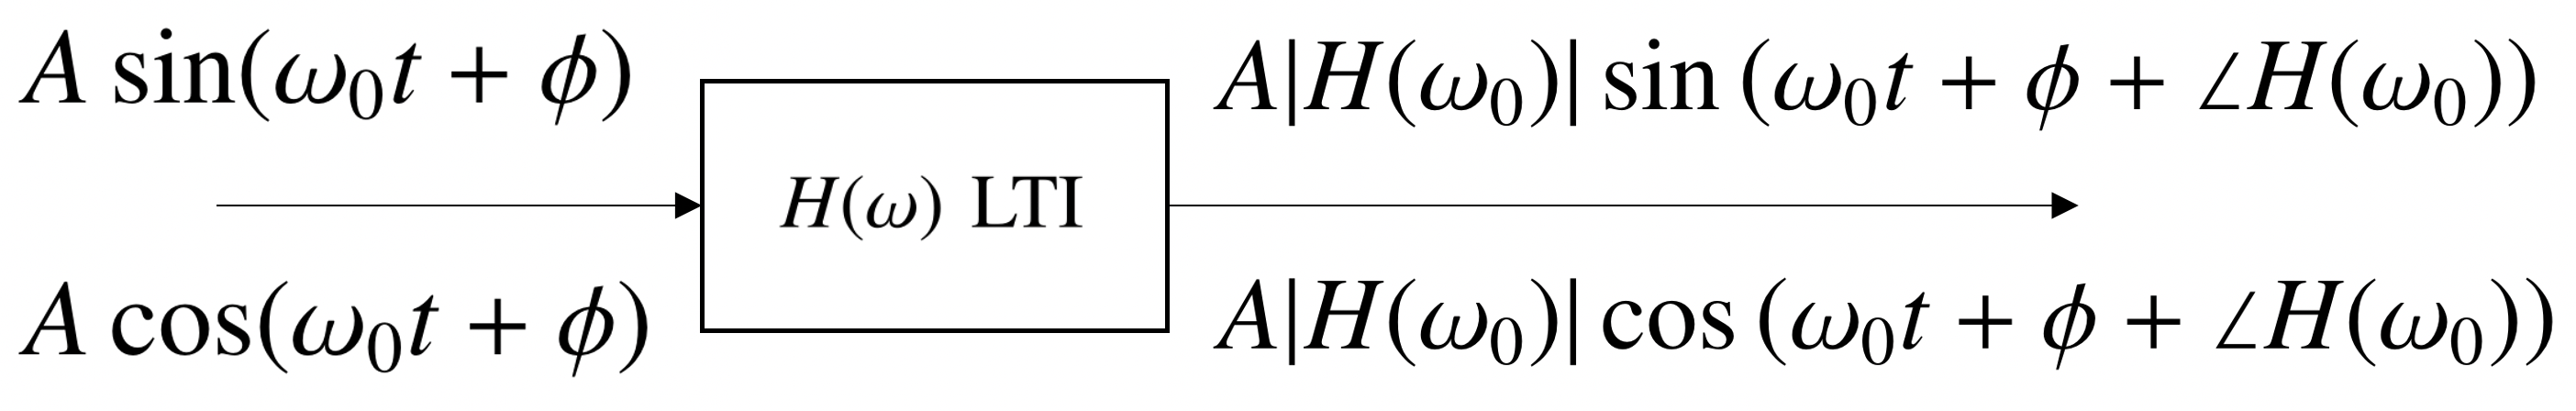
\includegraphics[width=6.3cm]{figure.png}
\end{figure}
Since perpendicular bisector of $\vec{x_1x_2}$ is perpendicular to $\vec{x_1x_2}$ and passes through $\vec{M}$, any general point $\vec{P}$ on the perpendicular bisector can be given using the relation
\begin{align}
    &\left(\vec{x_2}-\vec{x_1}\right)^\top\left(\vec{P}-\vec{M}\right)=0\\
    \implies &\left(\vec{x_2}-\vec{x_1}\right)^\top\vec{P}-\left(\vec{x_2}^\top-\vec{x_1}^\top\right)\left(\dfrac{\vec{x_1}+\vec{x_2}}{2}\right)=0\\
    \implies &\left(\vec{x_2}-\vec{x_1}\right)^\top\vec{P}=\dfrac{\vec{x_2}^\top\vec{x_2}-\vec{x_1}^\top\vec{x_1}+\vec{x_2}^\top\vec{x_1}-\vec{x_1}^\top\vec{x_2}}{2}
\end{align}
\end{frame}
\begin{frame}
Since $\vec{x_1}^\top\vec{x_2}=\vec{x_2}^\top\vec{x_1}$, the equation reduces to
\begin{align}
    2\left(\vec{x_2}-\vec{x_1}\right)^\top\vec{P}=\vec{x_2}^\top\vec{x_2}-\vec{x_1}^\top\vec{x_1}
\end{align}
Using \eqref{a}, we get
\begin{align}
    2\left(\vec{x_2}-\vec{x_1}\right)^\top\vec{P}&=-2\myvec{g&f}(\vec{x_2}-\vec{x_1})\\
    \implies \left(\vec{x_2}-\vec{x_1}\right)^\top\vec{P}&=\left(\vec{x_2}-\vec{x_1}\right)^\top\myvec{-g\\-f}
\end{align}
Since the centre of the circle is $\vec{C}=\myvec{-g\\-f}$, we can clearly see that $\vec{P}=\vec{C}$ satisfies the equation of perpendicular bisector.\\

Hence, the perpendicular bisector of any chord of a circle passes through the centre of the circle.
\end{frame}
\begin{frame}{Example}
For example, consider the circle
\begin{align}
    \vec{x}^\top\vec{x}+2\myvec{-4&-5}\vec{x}+5=0
\end{align}
and let $\vec{x_1}=\myvec{0\\5-2\sqrt{5}}$ and $\vec{x_2}=\myvec{-2\\5}$.
We can clearly see in the figure that the perpendicular bisector of the chord $\vec{x_1x_2}$ passes through the centre $\vec{C}$ of the circle.

\begin{figure}[h!]
    \centering
    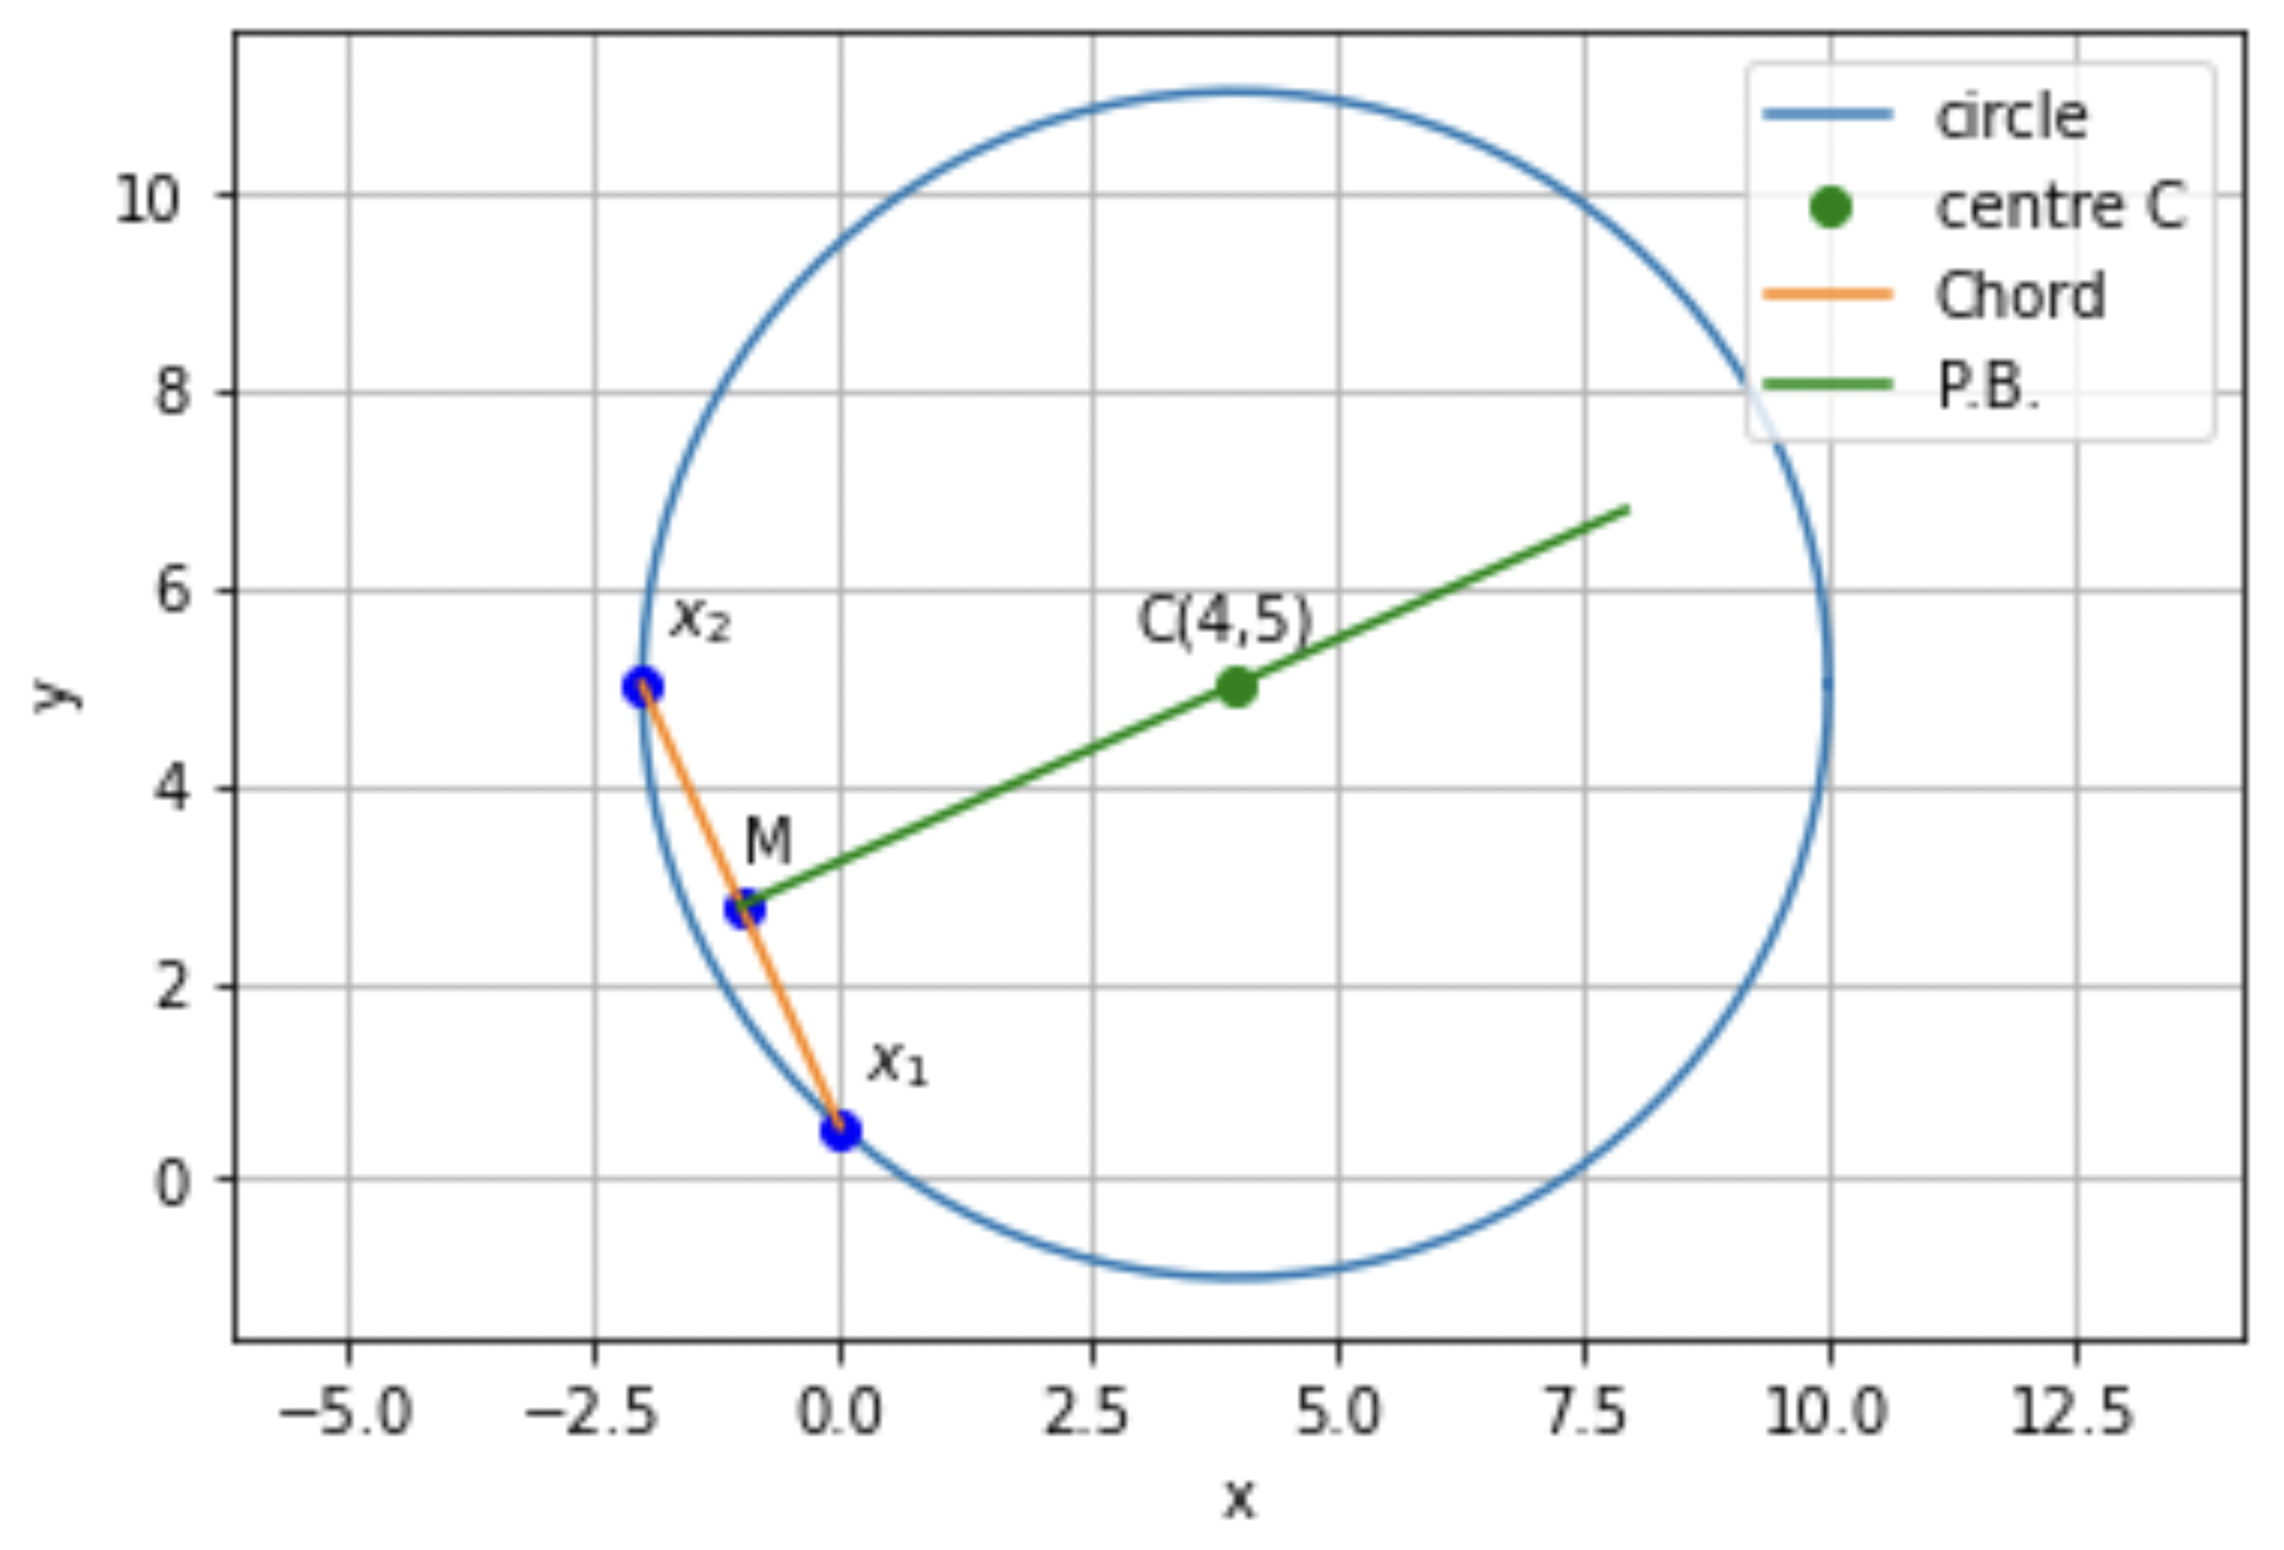
\includegraphics[width=6.3cm]{example_figure.png}
    \caption{Example figure}
\end{figure}
\end{frame}
\end{document}
